\documentclass[12pt,a4paper]{article}

\usepackage[bahasa]{babel}
\usepackage[margin=2.5cm]{geometry}
\usepackage{amsmath,amssymb}
\usepackage{graphicx}
\usepackage{hyperref}
\usepackage{enumitem}
\usepackage{booktabs}
\usepackage{float}
\usepackage{caption}
\usepackage{xcolor}
\usepackage{tcolorbox}
\usepackage{fancyhdr}
\usepackage{listings}
\usepackage{tocloft}

\geometry{margin=2.5cm}

\definecolor{primaryblue}{RGB}{25,55,109}
\definecolor{accentorange}{RGB}{230,126,34}
\definecolor{softbg}{RGB}{248,249,250}
\definecolor{codebg}{RGB}{245,245,250}
\definecolor{darkgreen}{RGB}{27,94,32}

\pagestyle{fancy}
\fancyhf{}
\fancyhead[L]{\small\textit{SiKandang --- Laporan UTS Basis Data 2}}
\fancyhead[R]{\small\thepage}
\fancyfoot[C]{}

\renewcommand{\contentsname}{DAFTAR ISI}
\addto\captionsindonesian{\renewcommand{\contentsname}{DAFTAR ISI}}

\lstset{
  backgroundcolor=\color{codebg},
  basicstyle=\ttfamily\small,
  breaklines=true,
  breakatwhitespace=true,
  frame=single,
  rulecolor=\color{primaryblue!25},
  showstringspaces=false,
  tabsize=2,
  keywordstyle=\color{primaryblue}\bfseries,
  commentstyle=\color{darkgreen},
  stringstyle=\color{accentorange!80!black},
  language=SQL,
  morekeywords={DELIMITER,TRIGGER,PROCEDURE,SIGNAL,RESIGNAL,TRANSACTION},
  captionpos=b
}

\newtcolorbox{infobox}{
  colback=softbg, colframe=primaryblue!40,
  arc=4pt, left=6pt, right=6pt, top=4pt, bottom=4pt
}
\newtcolorbox{warningbox}{
  colback=yellow!5, colframe=accentorange!60,
  arc=4pt, left=6pt, right=6pt, top=4pt, bottom=4pt
}

\hypersetup{
  colorlinks=true, linkcolor=primaryblue,
  urlcolor=primaryblue, citecolor=primaryblue
}

\begin{document}
\pagenumbering{arabic}

% ================= COVER =================
\begin{center}
\vspace*{1.2cm}
{\Large\bfseries\color{primaryblue} SiKandang}\\[0.3em]
{\large Aplikasi Pencatatan Pakan dan Panen Telur\\dengan Trigger dan Stored Procedure}\\[1.2em]
{\large Laporan Ujian Tengah Semester}\\[0.3em]
{\large Basis Data 2}\\[1.5em]
Diajukan untuk memenuhi penilaian Ujian Tengah Semester\\[0.3em]
Mata Kuliah Basis Data 2\\[1.5em]
Disusun oleh:\\[0.5em]
{\large Arfarizqhi Akbar \quad (462025611013)}\\[0.2em]
{\large Fatih Jawwad \quad (452024611047)}
{\large Universitas Darussalam Gontor}\\[0.2em]
{\large Program Studi Informatika}\\[0.2em]
{\large 2026}
\end{center}
\thispagestyle{plain}
\clearpage

% ================= TOC =================
\tableofcontents
\clearpage

% ================= 1 =================
\section{Pendahuluan}

SiKandang adalah aplikasi pencatatan pakan dan panen telur untuk peternakan ayam skala kecil. Aplikasi ini dibangun dengan PHP native di sisi backend, Tailwind CSS di sisi frontend, dan MariaDB (InnoDB) sebagai basis data. Fokus laporan ini adalah bagian basis data: bagaimana aturan bisnis yang kritis --- validasi stok dan pencatatan mutasi --- dipindahkan dari kode aplikasi ke dalam database melalui trigger dan stored procedure.

Keputusan desainnya sederhana. Stok pakan adalah angka yang tidak boleh salah. Jika validasi hanya ditulis di PHP, setiap jalur baru yang menyentuh tabel (CLI, Postman, skrip impor, endpoint baru) harus mengulang validasi yang sama, dan satu jalur yang lupa berarti stok bisa minus. Dengan menaruh validasi di trigger \texttt{BEFORE INSERT}, aturan tersebut melekat pada tabelnya: siapa pun yang mencoba mencatat pemberian pakan melebihi stok akan ditolak oleh database, lewat jalur apa pun. Trigger \texttt{AFTER INSERT} kemudian memotong stok dan menulis jejak auditnya, sedangkan stored procedure membungkus pencatatan pemberian pakan dan panen telur dalam satu transaksi atomik --- keduanya berhasil, atau keduanya batal.

Laporan ini mendokumentasikan skema basis data, dua trigger dan satu stored procedure yang diimplementasikan, diagram alur kerjanya, tutorial menjalankan aplikasi dari nol, serta skenario pengujian yang membuktikan bahwa mekanisme tersebut bekerja.

\begin{infobox}
\textbf{Prinsip desain:} stok \textbf{tidak pernah} diubah langsung oleh aplikasi. Semua pengurangan stok terjadi lewat trigger, sehingga validasi tidak bisa di-\textit{bypass} --- bahkan via CLI atau Postman.
\end{infobox}

% ================= 2 =================
\section{Skema Basis Data}

Basis data bernama \texttt{sikandang} dan terdiri dari empat tabel. Tabel \texttt{pakan} adalah master pakan sekaligus sumber kebenaran stok saat ini. Tabel \texttt{pemberian\_pakan} mencatat setiap pemberian pakan per kandang dan merupakan satu-satunya pintu masuk pengurangan stok. Tabel \texttt{panen\_telur} mencatat hasil panen dan terikat satu-satu ke pemberian pakan. Tabel \texttt{log\_stok\_pakan} adalah jejak audit setiap perubahan stok yang ditulis otomatis oleh trigger.

\begin{center}
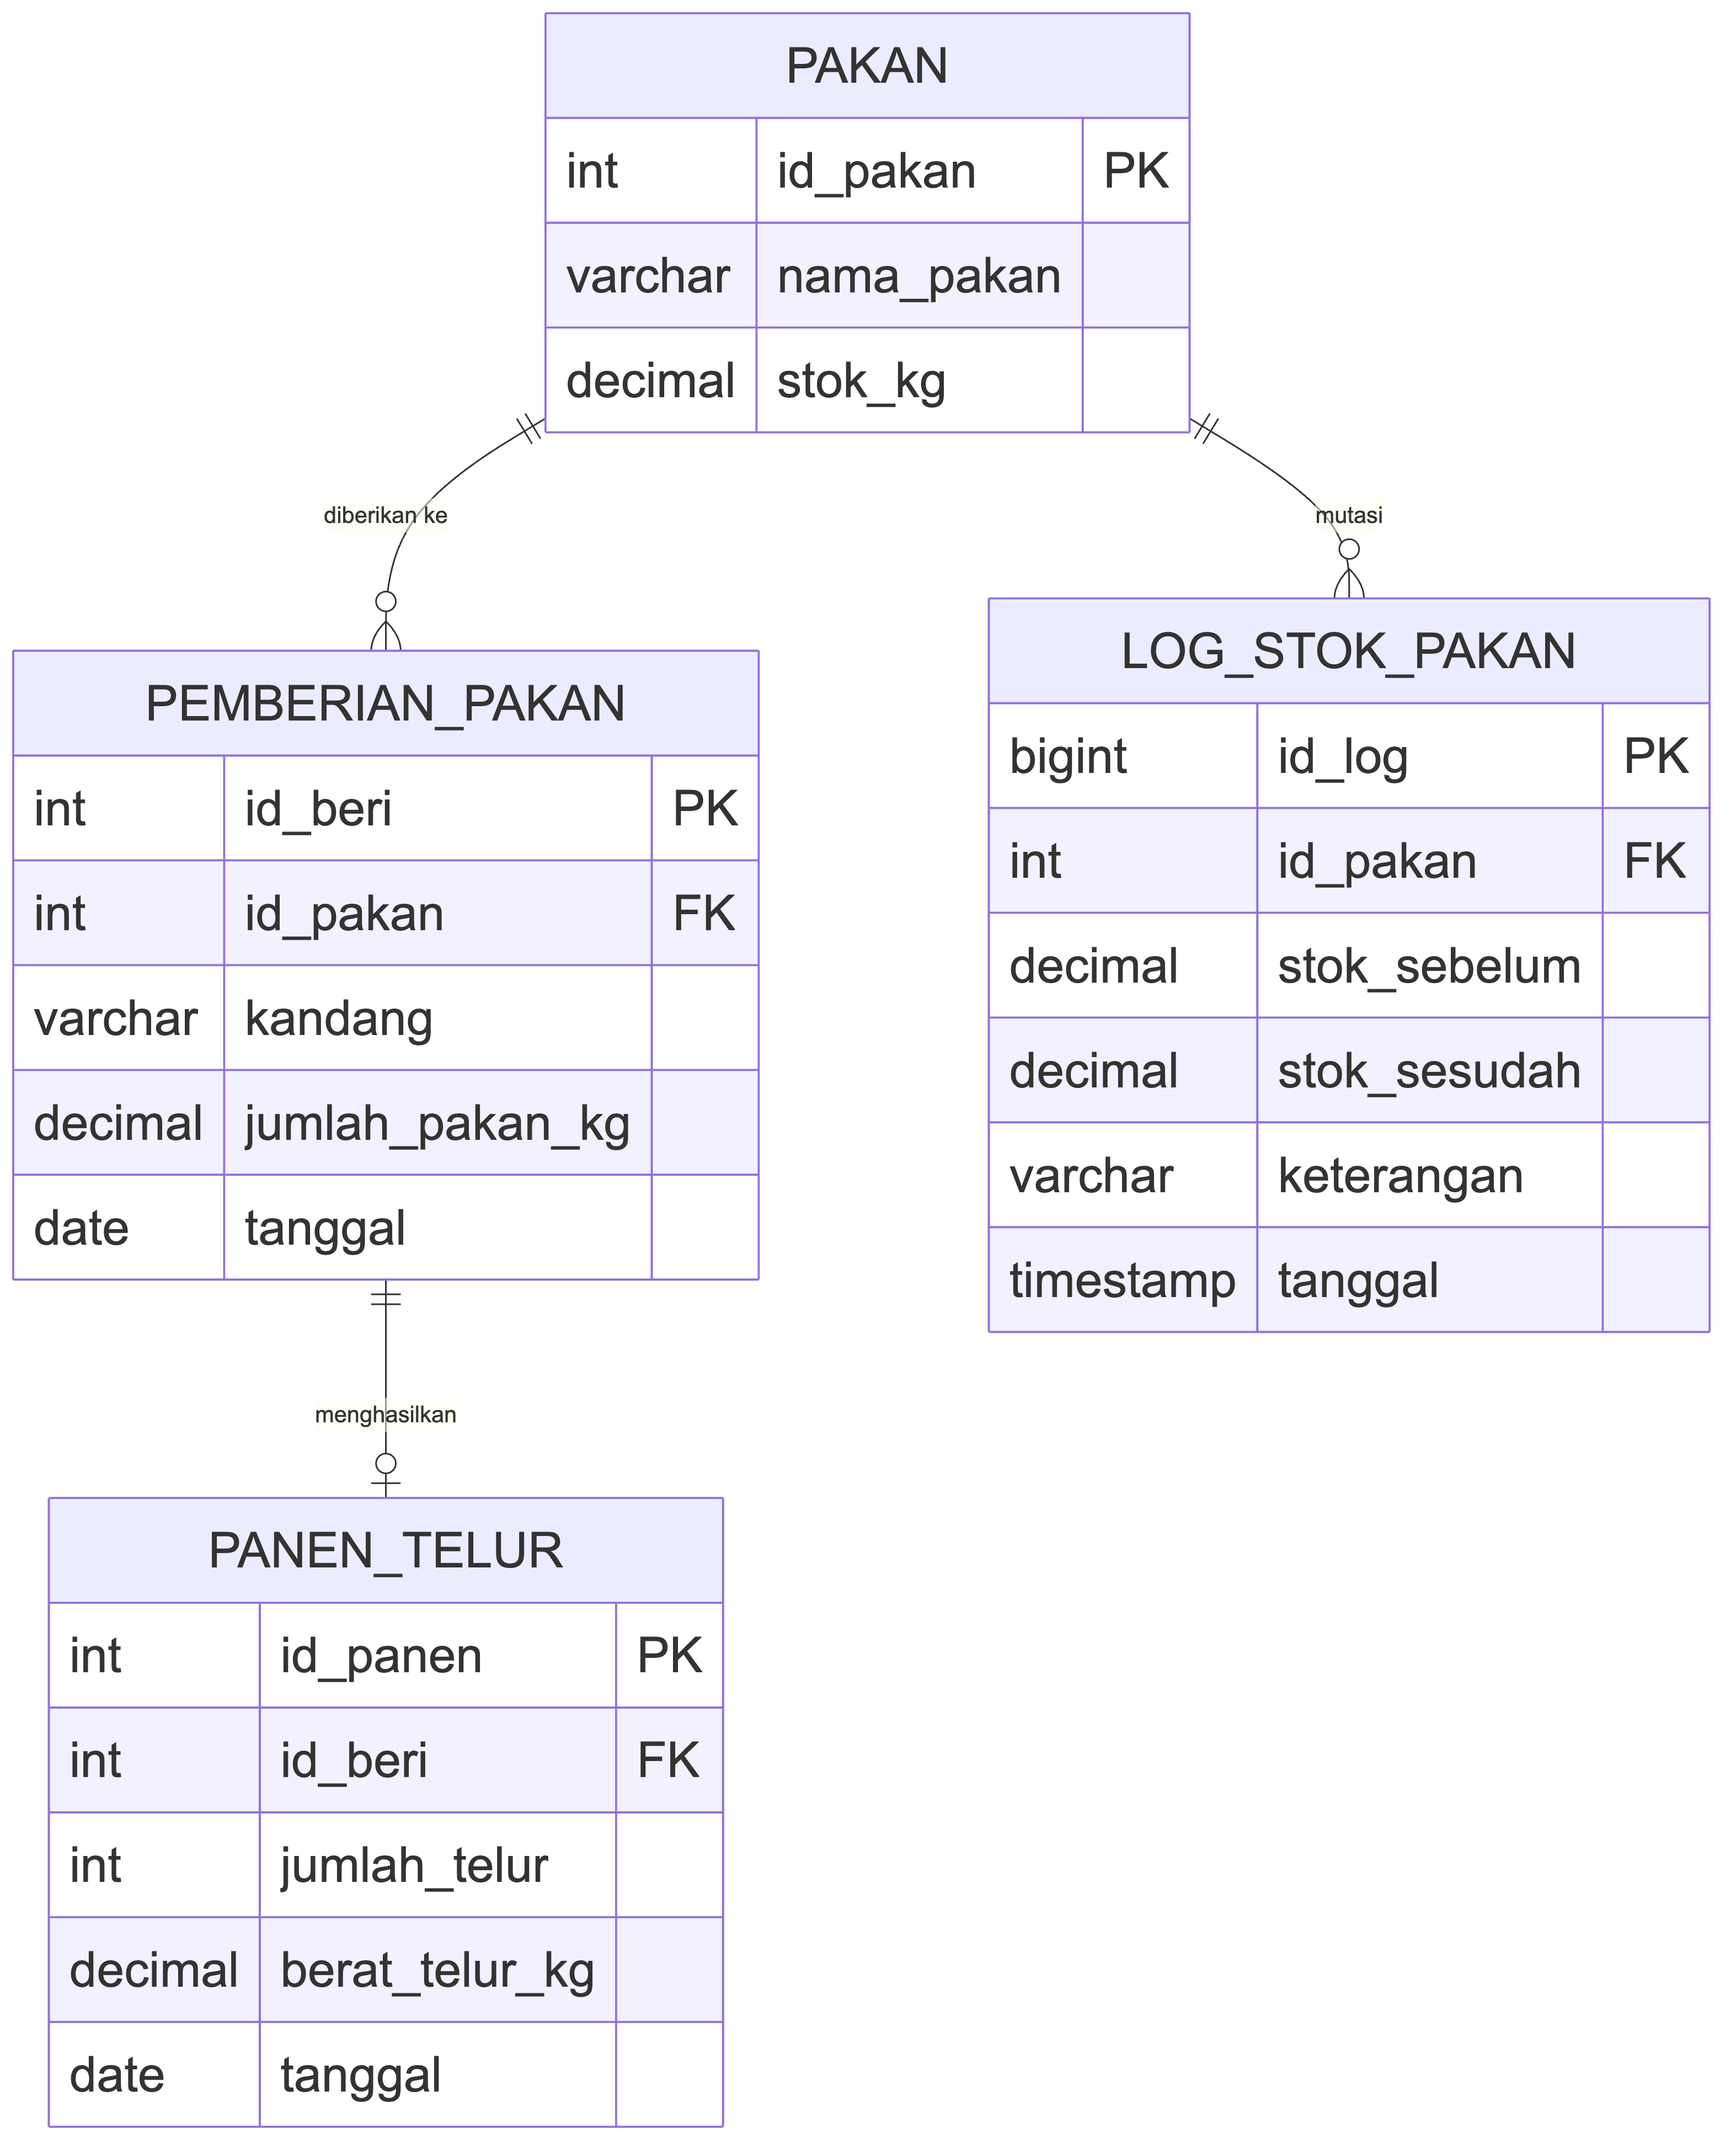
\includegraphics[width=0.85\textwidth,height=12.0cm,keepaspectratio]{fig-erd.png}
\captionof{figure}{Diagram relasi antar tabel SiKandang.}
\end{center}

\begin{table}[h]
\centering
\caption{Deskripsi tabel.}
\begin{tabular}{p{3.2cm} p{4.5cm} p{5.5cm}}
\toprule
\textbf{Tabel} & \textbf{Isi} & \textbf{Peran} \\
\midrule
\texttt{pakan} & Master pakan + stok saat ini & Sumber kebenaran stok \\
\texttt{pemberian\_pakan} & Riwayat pemberian per kandang & Diisi user, divalidasi trigger \\
\texttt{panen\_telur} & Hasil panen telur & Terikat 1:1 ke pemberian \\
\texttt{log\_stok\_pakan} & Jejak audit perubahan stok & Otomatis oleh trigger \\
\bottomrule
\end{tabular}
\end{table}

Relasinya: satu jenis pakan diberikan ke banyak kandang (\textit{many-to-one} dari \texttt{pemberian\_pakan} ke \texttt{pakan}); satu pemberian menghasilkan maksimal satu panen (\textit{one-to-one} antara \texttt{panen\_telur} dan \texttt{pemberian\_pakan}); satu pakan memiliki banyak riwayat mutasi (\textit{many-to-one} dari \texttt{log\_stok\_pakan} ke \texttt{pakan}). Seluruh tabel memakai engine InnoDB agar foreign key dan transaksi berfungsi, dengan constraint \texttt{CHECK} sebagai pertahanan lapis pertama (\texttt{stok\_kg >= 0}, \texttt{jumlah\_pakan\_kg > 0}).

% ================= 3 =================
\section{Trigger dan Stored Procedure}

\subsection{Ikhtisar objek}

\begin{table}[h]
\centering
\caption{Objek logika basis data yang diimplementasikan.}
\begin{tabular}{p{3.2cm} p{2.6cm} p{3.2cm} p{4.2cm}}
\toprule
\textbf{Objek} & \textbf{File} & \textbf{Timing} & \textbf{Fungsi} \\
\midrule
\texttt{trg\_cek\_pakan} & \texttt{03\_triggers.sql} & BEFORE INSERT pada \texttt{pemberian\_pakan} & Menolak INSERT jika stok kurang atau pakan tidak ada \\
\texttt{trg\_mutasi\_pakan} & \texttt{03\_triggers.sql} & AFTER INSERT pada \texttt{pemberian\_pakan} & Memotong stok dan mencatat ke \texttt{log\_stok\_pakan} \\
\texttt{sp\_catatan\_harian} & \texttt{04\_sp.sql} & Stored procedure & Menyimpan pemberian + panen dalam satu transaksi atomik \\
\bottomrule
\end{tabular}
\end{table}

\subsection{trg\_cek\_pakan --- validasi sebelum tulis}

Trigger ini berjalan setiap kali ada \texttt{INSERT} ke \texttt{pemberian\_pakan}, sebelum baris ditulis. Ia mengunci baris pakan terkait (\texttt{SELECT ... FOR UPDATE}) agar dua transaksi bersamaan tidak membaca stok yang sama, lalu memeriksa dua kondisi: pakan tidak ditemukan (\texttt{SIGNAL SQLSTATE '45000'}, pesan \texttt{pakan tidak ditemukan}) dan jumlah yang diminta melebihi stok (\texttt{SIGNAL SQLSTATE '45000'}, pesan \texttt{stok pakan tidak mencukupi}). Karena validasi hidup di database, endpoint PHP cukup meneruskan error 45000 sebagai respons HTTP 422 --- tidak ada logika stok di controller.

\begin{lstlisting}[caption={Trigger validasi stok (ringkas). File lengkap: backend/db/03\_triggers.sql.}]
CREATE TRIGGER trg_cek_pakan
BEFORE INSERT ON pemberian_pakan FOR EACH ROW
BEGIN
  DECLARE v_stok DECIMAL(10, 2);
  SELECT stok_kg INTO v_stok FROM pakan
    WHERE id_pakan = NEW.id_pakan FOR UPDATE;
  IF v_stok IS NULL THEN
    SIGNAL SQLSTATE '45000'
      SET MESSAGE_TEXT = 'pakan tidak ditemukan';
  ELSEIF NEW.jumlah_pakan_kg > v_stok THEN
    SIGNAL SQLSTATE '45000'
      SET MESSAGE_TEXT = 'stok pakan tidak mencukupi';
  END IF;
END
\end{lstlisting}

\subsection{trg\_mutasi\_pakan --- potong stok dan catat audit}

Setelah baris pemberian lolos validasi dan tersimpan, trigger ini memotong \texttt{pakan.stok\_kg} sebesar jumlah yang diberikan, lalu menulis satu baris ke \texttt{log\_stok\_pakan} berisi stok sebelum, stok sesudah, dan keterangan seperti \texttt{Pemberian \#12 - Kandang A1}. Aplikasi tidak pernah meng-\texttt{UPDATE} stok secara langsung; halaman riwayat stok (\texttt{GET /riwayat-stok}) murni membaca tabel log ini.

\subsection{sp\_catatan\_harian --- satu transaksi untuk dua tabel}

Mencatat pemberian pakan tanpa panen (atau sebaliknya) akan menghasilkan data yatim. Stored procedure \texttt{sp\_catatan\_harian} menerima enam parameter (kandang, id pakan, jumlah pakan, jumlah telur, berat telur, tanggal), membuka \texttt{START TRANSACTION}, memasukkan baris pemberian, mengambil id-nya via \texttt{LAST\_INSERT\_ID()}, memasukkan baris panen yang terikat ke id tersebut, lalu \texttt{COMMIT}. Jika langkah apa pun gagal --- termasuk penolakan oleh \texttt{trg\_cek\_pakan} --- handler \texttt{EXIT HANDLER FOR SQLEXCEPTION} melakukan \texttt{ROLLBACK} dan \texttt{RESIGNAL} agar PHP menerima pesan error aslinya. Repository PHP memanggilnya dengan satu baris: \texttt{CALL sp\_catatan\_harian(...)}.

% ================= 4 =================
\section{Alur Kerja}

\begin{center}
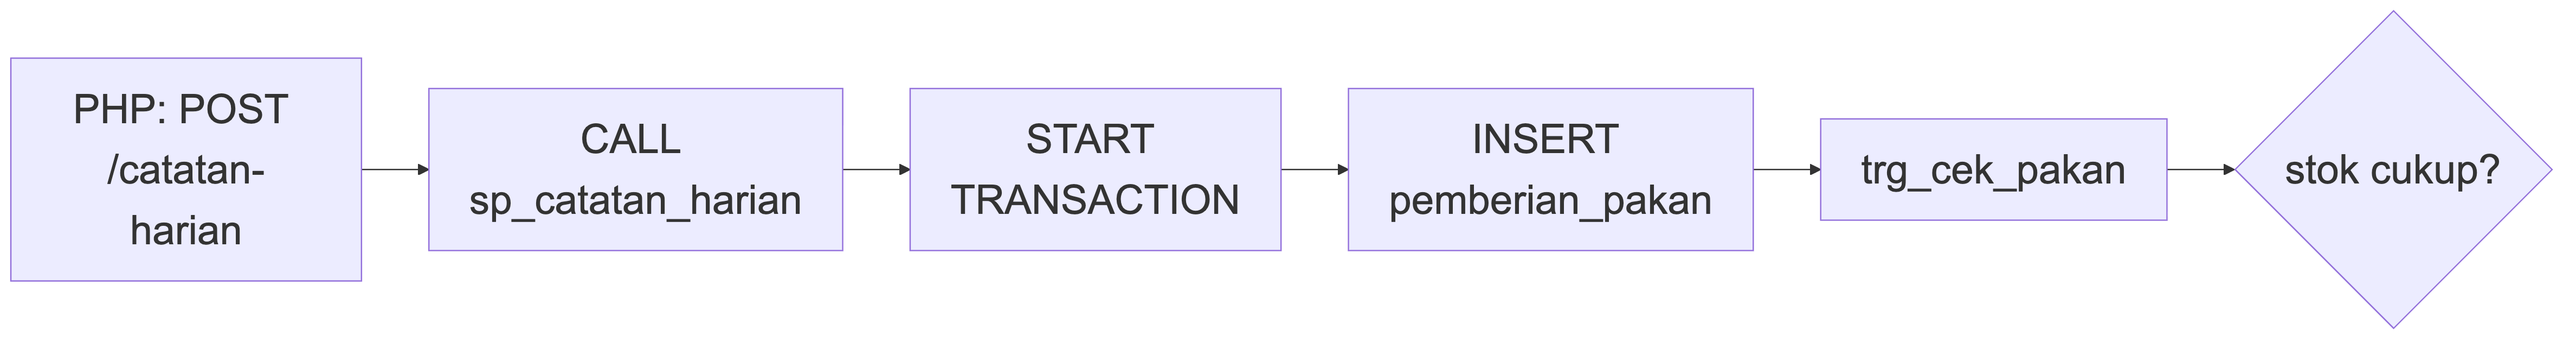
\includegraphics[width=\textwidth,height=4.0cm,keepaspectratio]{fig-alur1.png}
\vspace{2mm}
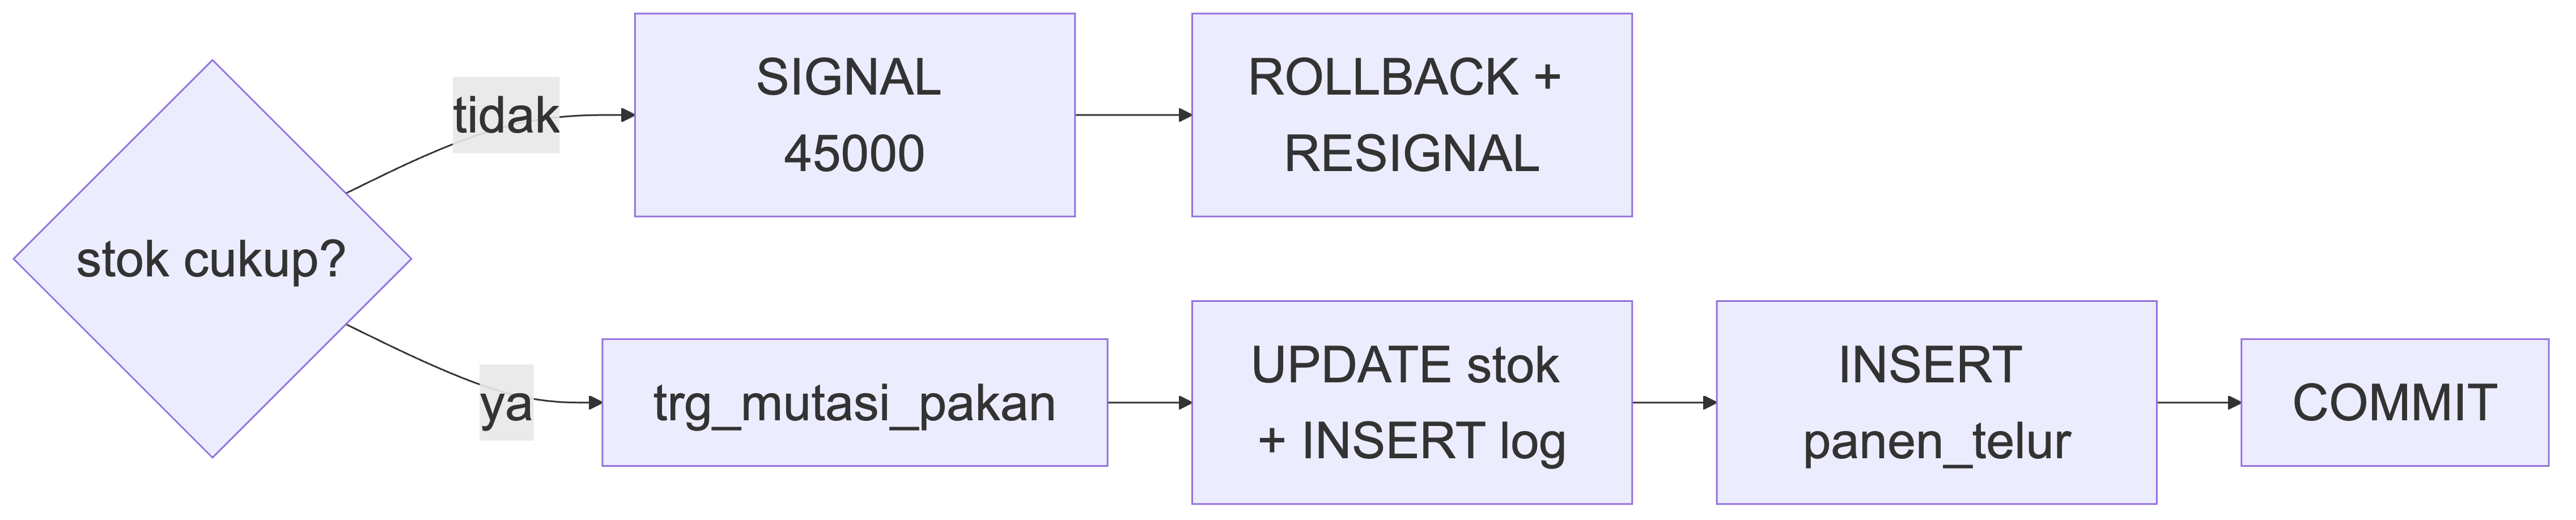
\includegraphics[width=\textwidth,height=5.0cm,keepaspectratio]{fig-alur2.png}
\captionof{figure}{Alur pencatatan harian dari request PHP hingga commit.}
\end{center}

Alurnya: request \texttt{POST /catatan-harian} divalidasi di PHP (format input), lalu memanggil \texttt{sp\_catatan\_harian} yang membuka transaksi. \texttt{INSERT} pemberian memicu \texttt{trg\_cek\_pakan}; jika stok tidak cukup, \texttt{SIGNAL 45000} menghentikan procedure, transaksi di-\textit{rollback}, dan error diteruskan ke PHP sebagai 422. Jika stok cukup, \texttt{trg\_mutasi\_pakan} memotong stok dan menulis log, baris panen dimasukkan, dan transaksi di-\textit{commit}. Perhatikan bahwa diagram ini adalah perbaikan dari versi sebelumnya yang gagal di-render GitHub karena sintaks label panah yang salah (\texttt{F -->|tidak --> G} tanpa penutup); versi yang benar memakai \texttt{F -->|tidak| G}.

% ================= 5 =================
\section{Tutorial Penggunaan}

\subsection{Prasyarat}

Dibutuhkan PHP, MariaDB, dan \texttt{just} (\url{https://github.com/casey/just}). Seluruh perintah dijalankan dari akar repositori.

\subsection{Instalasi}

\begin{lstlisting}[language=bash,caption={Instalasi dari nol.}]
git clone git@github.com:jaweed3/uts-web-dasar.git
cd uts-web-dasar
just db-setup
just serve
\end{lstlisting}

Perintah \texttt{just db-setup} berurutan membuat skema dan user database, mengisi data awal (3 jenis pakan: Konsentrat 100 kg, Bekatul 40 kg, Jagung Giling 75 kg), memasang trigger, lalu memasang stored procedure. Perintah \texttt{just serve} menjalankan server PHP di \texttt{http://localhost:8000}. File SQL juga dapat diimpor manual sesuai urutan: \texttt{01\_schema.sql}, \texttt{02\_seed.sql}, \texttt{03\_triggers.sql}, \texttt{04\_sp.sql} (file trigger/procedure memakai \texttt{DELIMITER //} di dalamnya dan diakhiri \texttt{DELIMITER ;}).

Perintah \texttt{just} lain yang tersedia: \texttt{just db-schema}, \texttt{just db-seed}, \texttt{just db-triggers}, \texttt{just db-sp}, \texttt{just db-test}, dan \texttt{just api-test}.

\subsection{Mencoba API}

\begin{lstlisting}[language=bash,caption={Melihat stok dan mencatat pemberian + panen.}]
# 1. Lihat daftar pakan dan stoknya
curl -s http://localhost:8000/sikandang/api/pakan

# 2. Catat pemberian 5 kg Konsentrat + panen 120 butir (stok cukup -> sukses)
curl -s -X POST http://localhost:8000/sikandang/api/catatan-harian \
  -H 'Content-Type: application/json' \
  -d '{"kandang":"A1","id_pakan":1,"jumlah_pakan_kg":5,
       "jumlah_telur":120,"berat_telur_kg":7.2,
       "tanggal":"2026-10-21"}'

# 3. Minta 999 kg (stok tidak cukup -> HTTP 422 berisi pesan trigger)
curl -s -X POST http://localhost:8000/sikandang/api/catatan-harian \
  -H 'Content-Type: application/json' \
  -d '{"kandang":"A1","id_pakan":1,"jumlah_pakan_kg":999,
       "jumlah_telur":120,"berat_telur_kg":7.2,
       "tanggal":"2026-10-21"}'

# 4. Lihat riwayat catatan dan riwayat stok
curl -s http://localhost:8000/sikandang/api/catatan-harian
curl -s http://localhost:8000/sikandang/api/riwayat-stok
\end{lstlisting}

Endpoint lengkap: \texttt{GET /pakan}, \texttt{GET /pakan/\{id\}}, \texttt{PUT /pakan/\{id\}}, \texttt{DELETE /pakan/\{id\}}, \texttt{GET /catatan-harian}, \texttt{POST /catatan-harian}, \texttt{GET /riwayat-stok} --- semuanya di bawah prefix \texttt{/sikandang/api}. Frontend statis tersedia di \texttt{frontend/} (halaman beranda, pakan, catatan harian, riwayat stok) dan memanggil endpoint yang sama.

\begin{warningbox}
\textbf{Cara membuktikan trigger tidak bisa di-bypass:} ulangi skenario stok-kurang langsung dari MariaDB CLI (\texttt{INSERT INTO pemberian\_pakan ... jumlah 999}), tanpa lewat PHP. Hasilnya sama --- error \texttt{stok pakan tidak mencukupi} --- karena validasi hidup di tabel, bukan di aplikasi.
\end{warningbox}

% ================= 6 =================
\section{Pengujian}

File \texttt{backend/db/05\_test.sql} berisi lima skenario yang dapat dijalankan via \texttt{just db-test}. Hasil yang diharapkan: (1) INSERT dengan stok cukup berhasil, stok berkurang, dan \texttt{log\_stok\_pakan} terisi; (2) INSERT 999 kg ditolak dengan pesan trigger, dan stok serta tabel tidak berubah; (3) \texttt{CALL sp\_catatan\_harian(...)} dengan stok cukup memasukkan pemberian, panen, dan log sekaligus; (4) procedure dengan jumlah 9999 kg gagal total --- \texttt{ROLLBACK} membuat \texttt{panen\_telur} tidak bertambah; (5) query gabungan tiga tabel yang dipakai endpoint \texttt{GET /catatan-harian} mengembalikan data yang konsisten.

% ================= 7 =================
\section{Link Repositori}

Kode program lengkap beserta dokumentasi basis data tersedia di:

\begin{center}
\url{https://github.com/jaweed3/uts-web-dasar} \\[0.3em]
Dokumentasi database: \url{https://github.com/jaweed3/uts-web-dasar/blob/master/backend/db/README.md}
\end{center}

Struktur direktori relevan: \texttt{backend/db/} (file \texttt{00\_users.sql} sampai \texttt{05\_test.sql}), \texttt{backend/src/} (controller, repository, koneksi database), \texttt{backend/public/} (routing API), dan \texttt{frontend/} (antarmuka pengguna).

\end{document}
